\section{Midlertidige løsninger}\label{sc:midlertidige}
Andre sikringer mod oversvømmelse placeres kun midlertidigt. Dette kan være fordi oversvømmelse sker sjældent i området, fordi eksisterende sikringer akut skal suppleres eller fordi en permanent sikring ville blokere trafik i dagligdagen \cite{fema2013}. Løsningerne anvendes til at sikre alt fra enkelte døråbninger til større beboelsesområder mod oversvømmelse \cite{barrierekatalog}. 
\par
Eksisterende midlertidige løsninger udgøres af lænsepumper og forskellige typer af barrierer. Blandt sidstnævnte tælles skillevægge, mobile dæmninger, luft- og vandslanger samt sandsækkediger. 
\\\\
\textbf{Lænsepumper} anvendes i forbindelse med oversvømmelser til at omdirigere vandmængderne. De bruges eksempelvis til at forebygge, at vand løber over dæmninger og diger \cite{morrison2012}. Lænsepumper skal kunne omdirigere store vandmængder over tid for at forebygge oversvømmelse ved skybrud eller stormfloder \cite{laensepumper}. Beredskabsstyrelsens pumper har eksempelvis en kapacitet, der spænder mellem 800 og 15.000 liter/minut \cite{brslaensepumper}. De store pumper kan have høje vandtryk, hvilket kan være farligt. Derfor kræver det trænet personale at implementere dem effektivt og sikkert \cite{safework2013}. Beredskabsstyrelsen udsender eksempelvis 6 personer per pumpe, herunder en holdleder, med deres største modeller \cite{brslaensepumper}.
\\\\
\textbf{Skillevægge} kan optræde som skotter, pudebarrierer, bjælkerækværker, boxwalls, eller andet \cite{barrierekatalog}. Som illustreret på Figur \ref{skillevaegge}, bliver de både brugt til at beskytte større områder og som mere præcise løsninger på enkelte vinduer, døre, skakte og lignende \cite{barrierguide2005}.

\begin{figure}[H]
    \centering
    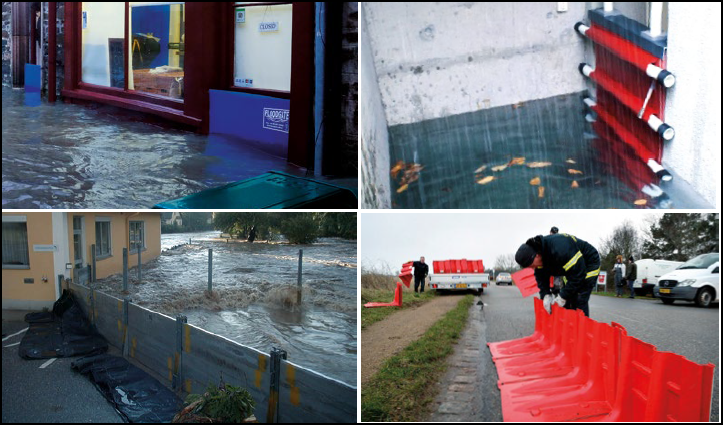
\includegraphics[width=0.7\textwidth]{figures/Skillevaegge.png}
    \caption{Øverst: Eksempel på et dørskot (t.v.) og en pudebarriere til en dør (t.h.). Nederst: Et rækværk fæstet med søjler (t.v.) og opsætning af en boxwall (t.h.) \cite{barrierekatalog}.}
    \label{skillevaegge}
\end{figure}

\textbf{Mobile dæmninger} optræder i oppusteligt format og placeres i vandområder, hvor der opstår et akut behov for at forebygge vandets gennemløb \cite{mobiledams}. De kan have en højde på 50 meter \cite{barrierekatalog}. Grundet løsningens størrelsesorden og prisleje implementeres den typisk af trænede professionelle \cite{fema2013}. 
\\\\
\textbf{Luft- og vandslanger} anvendes i stil med skillevægge og dæmninger til at blokere for vandets gennemløb \cite{flooddefensegroup}. De kan relativt nemt rulles kompakt sammen og transporteres, hvilket er en fordel i forhold til skillevægge og mobile dæmninger. Slangerne kan stabiliseres med omkransende skillevægge eller med kabler i jorden \cite{barrierekatalog}. For at undgå, at et hul i slangen fører til oversvømmelse, kan flere slanger ydermere splejses sammen, så der er mulighed for backup \cite{floodcontrolinternational}. 
\\\\
\textbf{Sandsækkediger} er en sidste mulighed blandt de midlertidige løsninger. Selve sækkenes anbefalede mål er ca. 40 x 85 cm, og de fremstilles ofte i materialerne jute eller nylon \cite{environmentagency2009}. De skal gerne fyldes med groft sand, men alternativt findes der sække på markedet med kemisk indhold, som udvider sig ved kontakt med vand \cite{barrierekatalog}. 
\par
Blandt alle de midlertidige løsninger er sandsække den, som oftest placeres af utrænet arbejdskraft \cite{fema2013}\cite{campbell2017}. Dette skyldes, at løsningen umiddelbart synes at være ligetil at implementere. Den kræver eksempelvis ikke transport af storgods eller evner til at betjene industrielle maskiner \cite{birch2018}. 
Sandsækkediger kan være effektive løsninger til at yde bred beskyttelse af et område mod vand og er ofte billigere end alternativerne \cite{environmentagency2009}. På landsbasis har Beredskabsstyrelsen ca. 1,3 millioner sandsække på lager \cite{brssandsaekke}. 
\par
Imidlertid er flere detaljer i placeringen af sandsækkene vigtige for, at digerne kan fungere optimalt. Eksempelvist skal lagene ideelt set ligge forskudt i forhold til hinanden, og åbningen på sandsækkene skal vende væk fra den retning, som vandet forventes at komme fra (se figur \ref{sandsaekkediger}) \cite{usarmysandbag}.

%%%%
\begin{figure}[H]
    \centering
    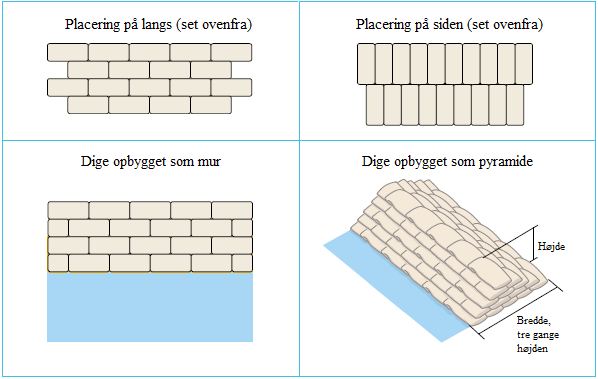
\includegraphics[width=0.7\textwidth]{figures/Sandsaekkediger.png}
    \caption{Øverst: Sandsækkene bør placeres forskudt, enten på langs (t.v.) eller på siden (t.h.). Nederst: Diget kan enten bygges op som en rektangulær "mur" (t.v.) eller som en pyramide med alternerende lag på langs og på siden (t.h.) \cite{environmentagency2009}.}
    \label{sandsaekkediger}
\end{figure}
%%%%

Der bliver ofte begået fejl i konstruktionen, når utrænede arbejdere bygger sandsækkediger. Fejlene kan skyldes uvidenhed, et højt stressniveau pga. akutte omstændigheder eller andet \cite{fema2013}\cite{campbell2017}. Ved fejl i konstruktionen kan der slippe større mængder af vand igennem diget, og i værste fald kan det styrte sammen, når vandet kommer \cite{environmentagency2009}. 
\par
En anden begrænsning ved brugen af sandsækkediger lægger sig til størrelsen på arbejdsbyrden uanset arbejdernes træningsniveau. Det tager gennemsnitligt 3 minutter for en almindelig person at fylde samt placere en enkelt sandsæk. Derudover tager det ca. 180 sække at bygge en 3 meter lang mur med en højde på 90 cm\cite{hutchison2018}. Det kræver altså en betydelig arbejdsindsats for mennesker at bygge digerne, hvis større områder skal sikres. Det sker endda, at arbejderne ikke når at blive færdige i tide, eller at de giver op pga. udmattelse, før digerne er høje nok \cite{campbell2017}. 
\par
På trods af, at sandsækkediger kan være effektive og har fordele over for andre løsninger, er der altså flere problemer med, hvordan de bliver implementeret i dag.

% Skal hænge sammen med, hvad der bliver sagt om de permanente løsninger
\subsection{Valg af en eksisterende løsning} 
Der er nu fundet begrænsninger ved en af de eksisterende løsninger. I opbygningen af sandsækkediger opstår der hændelige menneskelige fejl, og der er tale om en stor arbejdsbyrde med en høj grad af repetition. Disse mangler gør det relevant at overveje muligheder for automatisering. Der blev ikke fundet tilsvarende begrænsninger ved nogen af de andre løsninger, så disse vil ikke blive undersøgt yderligere.  
% Hvis vi ikke finder en tilsvarende begrænsning ved de andre løsninger, er der så brug for et mere udbygget argument? Den her konklusion virker måske tarvelig, når vi udsætter læseren for så mange spændende detaljer om forskellige former for diger, skillevægge mv.?
\par
% Iht. brugen inden for andre katastrofeområder. Skal hænge sammen med det pågældende afsnit.
Brugen af droneteknologi til bygning af sandsækkediger kunne lede til flere gevinster. Disse ligner dem, som gør sig gældende inden for andre katastrofeområder, hvor teknologien allerede anvendes (se kapitel \ref{sc:dronerkatastrofe}). % Ville være godt i hvert fald.
\par
Hvis droner for det første kunne garantere korrekt placering af sandsækkene ved eliminering af den menneskelige faktor, kunne en investering i teknologien give økonomiske besparelser over tid. Dette skyldes at der ville blive begået færre fejl i opbygningen af sandsækkedigerne end hidtil, og omkostninger forbundet med vandskader derfor oftere ville blive forhindret. 
\par
For det andet, kunne der drages nytte af, at droner ikke ligesom mennesker bliver langsommere til at arbejde ved stigende træthed (se afsnit \ref{sc:midlertidige} om sandsække). Flyvende droner har desuden mulighed for en nemmere arbejdsgang, hvis de kan nå frem til placeringsstedet med sækkene i fugleflugt i stedet for at navigere gennem terrænet. I denne type af scenarier kunne tilstrækkeligt høje sandsækkediger opbygges hurtigere. Dette ville give bygningen af sandsækkediger en højere succesrate og flere mulige use cases.
\par
For det tredje, kunne en automatisering af opgaven frigøre professionel og frivillig arbejdskraft, som kunne være til nytte andetsteds. Dette kunne være i forbindelse med evakueringen, den humanitære indsats, i implementeringen af sikringer med behov for professionel arbejdskraft (se afsnit \ref{sc:midlertidige} om sandsække) eller andet. Automatiseringen tænkes altså at være til mulig gavn, fordi frigjort arbejdskraft kunne forbedre kvaliteten af katastrofeindsatsen som helhed.
\par

% Lidt om feasibility (versat: "realistisk mulig"). Skal kunne spille sammen med, at vi har et afsnit i implementeringen, som behandler nogle af de samme emner. Evt. helt flyttes derned i stedet for?
\subsection{Løsningens realiserbarhed} 
Automatisering i denne sammenhæng tænkes at være realistisk mulig af flere grunde. \\
Omkostningerne ved oversvømmelser er for det første tilstrækkeligt store til, at selv en investering i dyr droneteknologi kunne betale sig (se kapitel \ref{sc:oversvoemmelser}). Disse omkostninger forudses som nævnt at blive større i fremtiden. 
\par
Det ligger også inden for mulighedernes rammer, at droner ville være i stand til at transportere sandsækkene rundt. Der eksisterer allerede nu flyvende droner, som kan løfte flere hundrede kilogram ad gangen, så det synes rimeligt at antage, at droner også kunne flytte rundt på sandsække, der typisk vejer 15 kg per styk \cite{aerones}\cite{usarmysandbag}. 
\par
Nutidige droner har kort batteritid i forhold til omfanget af opgaven at bygge sandsækkediger. Den højeste kapacitet for flyvende droner ligger eksempelvis på ca. 30 minutter, og den er endnu mindre ved de større modeller \cite{flynt2019}. Behov for opladninger under opbygningen af diget kunne mindske arbejdets effektivitet betydeligt. Imidlertid kunne denne udfordring potentielt overkommes. En ligefrem tilgang kunne eksempelvis være blot at opjustere antallet af droner til arbejdet eller medbringe ekstra batterier, så der er mulighed for løbende udskiftning, hvis dronerne løber tør for strøm. 
\par
Der var som tidligere nævnt særlige krav til sandsækkenes placering i forhold til hinanden (se afsnit \ref{sc:midlertidige} om sandsække). Det er også realistisk muligt, at droner kunne løse dette problem, eksempelvis ved brug af mønstergenkendelsesalgoritmer. Med nutidig teknologi kan der allerede skelnes mellem forskellige menneskelige ansigter \cite{patternrec}. Det synes derfor rimeligt at antage, at en mønstergenkendelsesalgoritme kunne identificere en sandsæks position, evt. med særlige markører anbragt på objektet. 
% Flere grunde..?
\par
På grund af de mulige gevinster og argumenterne for løsningens realiserbarhed, vil dette projekt undersøge mulighederne for at automatisere bygning af sandsækkediger ved brug af droneteknologi.